\section{Supplementary}
\label{sec:supplementary}

\subsection{Where EFO places height, weight, and BMI}
\label{sec:supp-figure}

Body mass index is defined by two other traits. The Experimental Factor Ontology says so itself: its textual definition of \texttt{body mass index} reads "An indicator of body density as determined by the relationship of BODY WEIGHT to BODY HEIGHT. BMI=weight (kg)/height squared (m2)" \citep{efo_malone2010}. That dependency appears in the free text, where nothing can compute on it, and nowhere in the ontology's structure.

Figure \ref{fig:efo_bmi_tree} shows the consequence. The two arguments of the same function sit at opposite extremes of the hierarchy.

\begin{figure}[htbp]
  \centering
  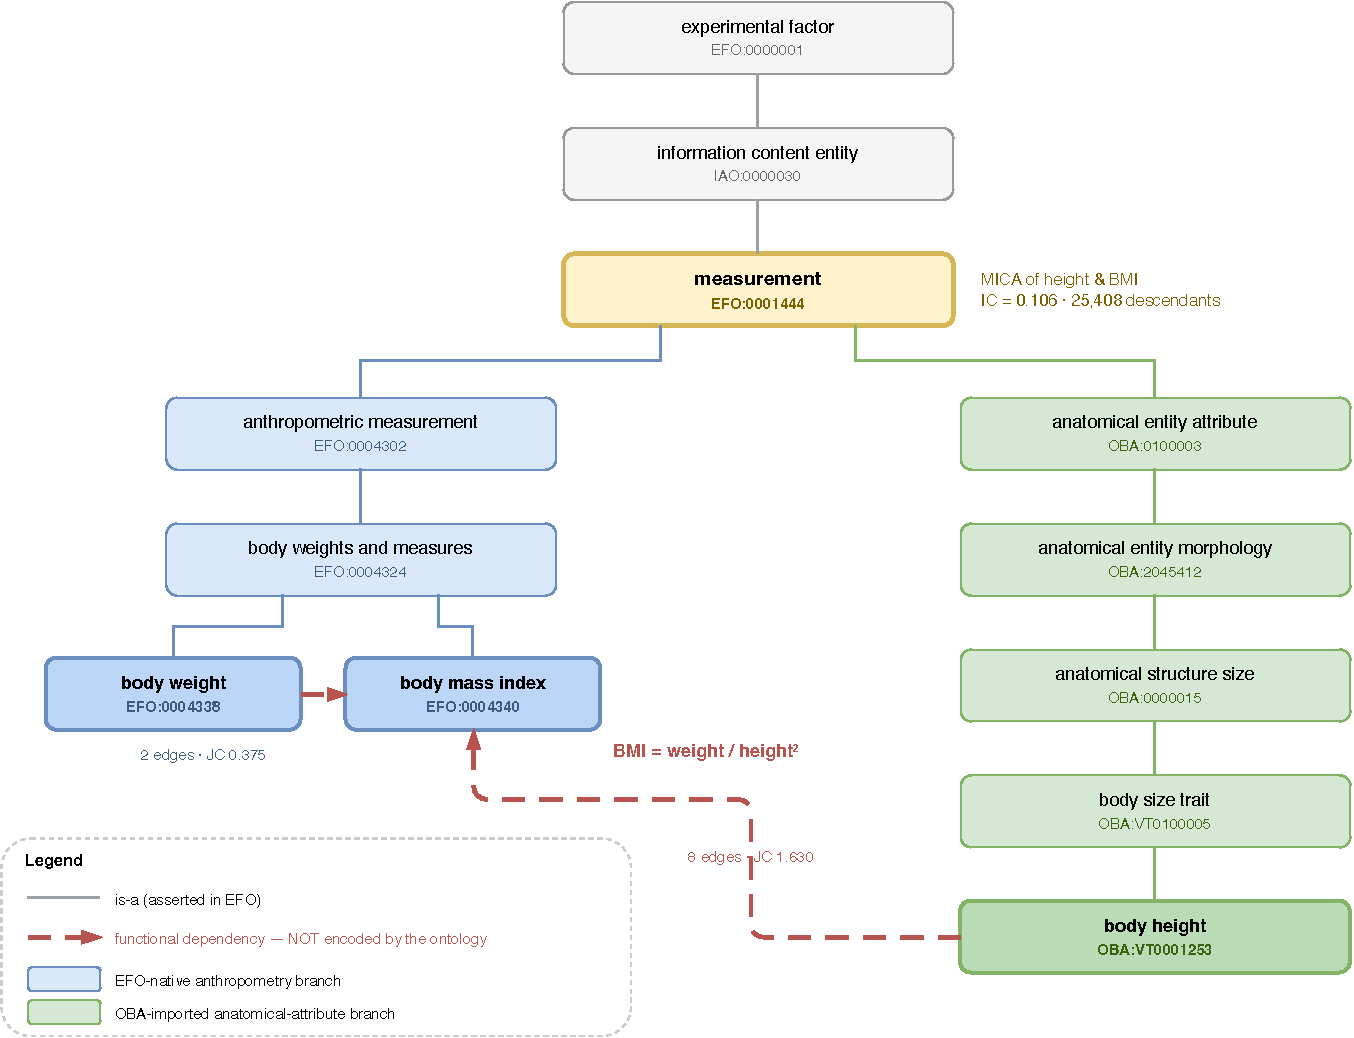
\includegraphics[width=\textwidth]{figures/efo_bmi_tree.pdf}
  \caption{Body height, body weight, and body mass index in EFO. Solid lines
  are asserted \texttt{is-a} edges; dashed lines are the functional dependency
  $\mathrm{BMI} = \mathrm{weight}/\mathrm{height}^{2}$, which EFO states in
  prose but does not encode. \emph{Body weight} is a sibling of BMI, two edges
  away; \emph{body height} is eight edges away across a branch imported from
  the Ontology of Biological Attributes. Their most informative common
  ancestor is \emph{measurement}, a class general enough to subsume 25{,}408
  of the ontology's 84{,}372 terms.}
  \label{fig:efo_bmi_tree}
\end{figure}

The asymmetry has no semantic justification. It follows from curation lineage: \texttt{body weight} is native EFO anthropometry, whereas \texttt{body height} is imported from OBA and inherits that ontology's anatomical-attribute spine.

\subsection{Structural separation}
\label{sec:supp-structure}

The following quantities depend on nothing but the asserted hierarchy. They involve no corpus, no probability model, and no free parameters; the last column is the Wu--Palmer similarity \citep{wu1994}.

\begin{table}[htbp]
\centering
\small
\begin{tabularx}{\textwidth}{|>{\raggedright\arraybackslash}X|>{\raggedright\arraybackslash}X|>{\raggedright\arraybackslash}X|>{\raggedright\arraybackslash}X|>{\raggedright\arraybackslash}X|}
\hline
\textbf{Pair} & \textbf{Most informative common ancestor} & \textbf{Classes it subsumes} & \textbf{Shortest path} & \textbf{Wu--Palmer} \\
\hline
BMI -- body weight & body weights and measures (EFO:0004324) & 40 & 2 edges & 0.800 \\
BMI -- body height & measurement (EFO:0001444) & 25,408 & 8 edges & 0.333 \\
\hline
\end{tabularx}
\end{table}

The middle column is the most direct statement of the problem. Two traits join under a class covering 40 of the ontology's 84,372 terms; the other pair joins only under a class covering 25,408 of them --- a 635-fold difference in the generality of the junction. Whatever "similar" is taken to mean, BMI and body height share little more than both being measurements.

\subsection{Information content, and why it is reported second}
\label{sec:supp-ic}

No annotation corpus is assumed here, so information content must be derived from structure. Using the intrinsic formulation of Seco et al. \citep{seco2004}, $\mathrm{IC}(c) = 1 - \log(|\mathrm{desc}(c)|+1) / \log N$ over the $N = 84{,}372$ classes beneath \texttt{experimental factor}:

\begin{table}[htbp]
\centering
\small
\begin{tabularx}{\textwidth}{|>{\raggedright\arraybackslash}X|>{\raggedright\arraybackslash}X|>{\raggedright\arraybackslash}X|>{\raggedright\arraybackslash}X|>{\raggedright\arraybackslash}X|}
\hline
\textbf{Class} & \textbf{CURIE} & \textbf{Descendants} & \textbf{Depth} & \textbf{Intrinsic IC} \\
\hline
measurement & EFO:0001444 & 25,408 & 2 & 0.106 \\
body weights and measures & EFO:0004324 & 40 & 4 & 0.673 \\
body mass index & EFO:0004340 & 5 & 5 & 0.842 \\
body weight & EFO:0004338 & 3 & 5 & 0.878 \\
body height & OBA:VT0001253 & 0 & 7 & 1.000 \\
\hline
\end{tabularx}
\end{table}

Similarity is reported under the three standard information-theoretic measures \citep{resnik1995,lin1998,jiang1997}.

\begin{table}[htbp]
\centering
\small
\begin{tabularx}{\textwidth}{|>{\raggedright\arraybackslash}X|>{\raggedright\arraybackslash}X|>{\raggedright\arraybackslash}X|>{\raggedright\arraybackslash}X|}
\hline
\textbf{Pair} & \textbf{Resnik} & \textbf{Lin} & \textbf{Jiang--Conrath distance} \\
\hline
BMI -- body weight & 0.673 & 0.782 & 0.375 \\
BMI -- body height & 0.106 & 0.115 & 1.630 \\
\hline
\end{tabularx}
\end{table}

These figures agree with the structural ones --- the separation is roughly fourfold on every measure, and remains so under the depth-blended intrinsic IC of Zhou et al. \citep{zhou2008} --- but they are reported second, and with three caveats, because intrinsic IC is a weaker instrument than its name suggests.

First, it is not $-\log p(c)$ for any distribution, so the information-theoretic reading of Jiang--Conrath as "information not shared", and its metric properties, do not transfer.

Second, it saturates at leaves. Every leaf receives $\mathrm{IC} = 1$ regardless of depth, so the value 1.000 for \texttt{body height} records only that nothing sits beneath it.

Third, and most damaging in this context, descendant count measures curation volume rather than generality. BMI scores as \textit{less} informative than body weight (0.842 against 0.878) solely because five subclasses have been curated beneath it and only three beneath body weight. A statistic derived from the hierarchy inherits exactly the curation artefacts that this paper is about. It cannot be the primary evidence that those artefacts exist.

\subsection{No corpus can equalise the two pairs}
\label{sec:supp-proposition}

The natural objection is that intrinsic IC is the wrong instrument and that a genuine annotation corpus --- the GWAS Catalog, for which EFO is the annotation vocabulary --- would place BMI symmetrically between its two arguments. It would not. The obstruction is structural, and no choice of corpus removes it.

Write $\mathcal{A}(x)$ for the ancestors of $x$ including $x$ itself, and let $h$, $w$, $b$ denote body height, body weight, and body mass index. From the asserted hierarchy,

\begin{equation}
\label{eq:ca-subset}
\mathcal{A}(h) \cap \mathcal{A}(b)
\;=\; \{\,\textrm{ICE},\; \textrm{experimental factor},\; \textrm{measurement}\,\}
\;\subsetneq\;
\mathcal{A}(w) \cap \mathcal{A}(b),
\end{equation}

the larger set additionally containing \texttt{anthropometric measurement} and \texttt{body weights and measures}. The inclusion is strict.

Under the standard construction, $p(c)$ is the share of annotations falling on $c$ or any of its descendants. Every instance of a class is an instance of its subsumers, so for any corpus whatsoever,

\begin{equation}
\label{eq:antimono}
c \sqsubseteq d \;\Longrightarrow\; p(c) \le p(d) \;\Longrightarrow\; \mathrm{IC}(c) \ge \mathrm{IC}(d).
\end{equation}

This is a consequence of subsumption semantics, not of the data. Resnik similarity is a maximum of IC over the common ancestors,

\begin{equation}
\label{eq:resnik}
\mathrm{sim}_{\mathrm{Res}}(x,y) \;=\; \max_{c \,\in\, \mathcal{A}(x) \cap \mathcal{A}(y)} \mathrm{IC}(c),
\end{equation}

and a maximum over a subset cannot exceed the maximum over its superset. Combining this with (\ref{eq:ca-subset}) gives the following.

\textbf{Proposition.} For every annotation corpus, $\mathrm{sim}_{\mathrm{Res}}(h, b) \le \mathrm{sim}_{\mathrm{Res}}(w, b)$. The inequality is strict whenever body height receives at least one annotation.

\textit{Proof.} The inequality is immediate from (\ref{eq:ca-subset}), (\ref{eq:antimono}) and (\ref{eq:resnik}). For strictness, note that \texttt{body height} is subsumed by \texttt{measurement} but not by \texttt{body weights and measures}, so the two subtrees are disjoint and $p(\textrm{measurement}) \ge p(\textrm{body weights and measures}) + p(h)$. If $p(h) > 0$ the inequality is strict, hence $\mathrm{IC}(\textrm{measurement}) < \mathrm{IC}(\textrm{body weights and measures})$, and these are the two maxima in question. $\square$

Set-based variants inherit the same obstruction, since they aggregate IC over an ancestor intersection that is strictly smaller for the height pair.

Lin and Jiang--Conrath divide by the information content of the leaves, which does depend on the corpus, so formal equality is reachable for them. The price makes the point. Solving for the corpus that equalises Lin under otherwise plausible annotation frequencies requires $p(\textrm{body weight}) \approx 5 \times 10^{-12}$: body weight would have to be roughly a billion times rarer than body height in the annotation record. Such a corpus does not describe genetics, and even then it achieves equality by cancelling a structural asymmetry against a frequency asymmetry, leaving the junction itself exactly where it was.

\subsection{Scope of the claim}
\label{sec:supp-scope}

The result is about reweighting, not about evidence in general. A corpus assigns mass to the nodes of a subsumption lattice; it cannot add an edge to that lattice. Because $\mathrm{BMI} = \mathrm{weight}/\mathrm{height}^{2}$ is symmetric in its two arguments while the lattice is not, no distribution over the lattice can recover the symmetry. The limitation is therefore not a deficiency of EFO's curation, which better annotation would repair, but a ceiling on what subsumption hierarchies can express.

The claim is correspondingly bounded. It says nothing against ontologies that assert non-taxonomic relations: an explicit \texttt{has\_input} or \texttt{derives\_from} edge from BMI to its two arguments would be traversable by a relation-aware measure, and would restore the symmetry directly. What cannot be repaired by evidence is a missing relation \textit{type}. That is the gap the compositional construction of Section \ref{sec:methods} is intended to fill.
